%%%%%%%%%%%%%%%%%%%%%%%%%%%%%%%%%%%%%%%%%%%%%%%%%%%%%%%%%%%%%%%%%%%%%%%%%%%%%%%%%%%%%%
% Modelo de relatório de Disciplina de MLP a partir da
% classe latex iiufrgs disponivel em http://github.com/schnorr/iiufrgs
%%%%%%%%%%%%%%%%%%%%%%%%%%%%%%%%%%%%%%%%%%%%%%%%%%%%%%%%%%%%%%%%%%%%%%%%%%%%%%%%%%%%%%

% Ignore o comentario acima e imagine que exista um modelo de relatorio de CCI em algum lugar

%%%%%%%%%%%%%%%%%%%%%%%%%%%%%%%%%%%%%%%%%%%%%%%%%%%%%%%%%%%%%%%%%%%%%%%%%%%%%%%%%%%%%%
% Definição do tipo / classe de documento e estilo usado
%%%%%%%%%%%%%%%%%%%%%%%%%%%%%%%%%%%%%%%%%%%%%%%%%%%%%%%%%%%%%%%%%%%%%%%%%%%%%%%%%%%%%%
%
\documentclass{iiufrgs}

%%%%%%%%%%%%%%%%%%%%%%%%%%%%%%%%%%%%%%%%%%%%%%%%%%%%%%%%%%%%%%%%%%%%%%%%%%%%%%%%%%%%%%
% Importação de pacotes
%%%%%%%%%%%%%%%%%%%%%%%%%%%%%%%%%%%%%%%%%%%%%%%%%%%%%%%%%%%%%%%%%%%%%%%%%%%%%%%%%%%%%%
% (a A seguir podem ser importados os pacotes necessários para o documento, de acordo 
% com a necessidade)
%
\usepackage[brazilian]{babel}	    % para texto escrito em pt-br
\usepackage[utf8]{inputenc}         % pacote para acentuação
\usepackage{graphicx}         	    % pacote para importar figuras
\usepackage[T1]{fontenc}            % pacote para conj. de caracteres correto
\usepackage{times}                  % pacote para usar fonte Adobe Times
\usepackage{enumerate}              % para lista de itens com letras
\usepackage{breakcites}
\usepackage{caption}
\usepackage{siunitx}
\usepackage{placeins}
\usepackage{titlesec}
\usepackage{enumitem}
\usepackage{titletoc}
\usepackage{epigraph}
\usepackage{subfig}
\usepackage{csquotes}
%\usepackage{listings}			    % para listagens de código-fonte
\usepackage{mathptmx}               % p/ usar fonte Adobe Times nas formulas matematicas
\usepackage{url}                    % para formatar URLs
%\usepackage{color}				    % para imagens e outras coisas coloridas
%\usepackage{fixltx2e}              % para subscript
%\usepackage{amsmath}               % para \epsilon e matemática
%\usepackage{amsfonts}
%\usepackage{setspace}			    % para mudar espaçamento dos parágrafos
%\usepackage[table,xcdraw]{xcolor}  % para tabelas coloridas
%\usepackage{longtable}             % para tabelas compridas (mais de uma página)
%\usepackage{float}
%\usepackage{booktabs}
%\usepackage{tabularx}
%\usepackage{hyperref}

\usepackage[alf,abnt-emphasize=bf]{abntex2cite}	% pacote para usar citações abnt

%%%%%%%%%%%%%%%%%%%%%%%%%%%%%%%%%%%%%%%%%%%%%%%%%%%%%%%%%%%%%%%%%%%%%%%%%%%%%%%%%%%%%%
% Macros, ajustes e definições
%%%%%%%%%%%%%%%%%%%%%%%%%%%%%%%%%%%%%%%%%%%%%%%%%%%%%%%%%%%%%%%%%%%%%%%%%%%%%%%%%%%%%%
%

% define estilo de parágrafo para citação longa direta:
\newenvironment{citacao}{
    %\singlespacing
    %\footnotesize
    \small
    \begin{list}{}{
        \setlength{\leftmargin}{4.0cm}
        \setstretch{1}
        \setlength{\topsep}{1.2cm}
        \setlength{\listparindent}{\parindent}
    }
    \item[]}{\end{list}
}

% adiciona a fonte em figuras e tabelas
\newcommand{\fonte}[1]{\\Fonte: {#1}}

\newcommand{\titlepagespecificinfo}{Relatório apresentado como requisito parcial para a obtenção de conceito na disciplina de Métodos Ágeis.}

% Ative o seguinte caso alguma nota de rodapé fique muito longa e quebre entre múltiplas
% páginas
%\interfootnotelinepenalty=10000

%%%%%%%%%%%%%%%%%%%%%%%%%%%%%%%%%%%%%%%%%%%%%%%%%%%%%%%%%%%%%%%%%%%%%%%%%%%%%%%%%%%%%%
% Informações gerais                                   
%%%%%%%%%%%%%%%%%%%%%%%%%%%%%%%%%%%%%%%%%%%%%%%%%%%%%%%%%%%%%%%%%%%%%%%%%%%%%%%%%%%%%%

% título
\title{REUNIÕES RETROSPECTIVAS EM SCRUM NA PERSPECTIVA DO SCRUMMASTER} 

% autor
%\author{Autores(s)}{Aluno(s)} % {sobrenome}{nome}
\author{Corrêa Pereira da Silva}{Henrique}

% Professor orientador da disciplina
\advisor[Profª.~Dra.]{Becker}{Karin}

% Nome do(s) curso(s):
\course{Curso de Graduação em Ciência da Computação}

% local da realização do trabalho 
\location{Porto Alegre}{RS} 

% data da entrega do trabalho (mês e ano)
\date{6}{2018}


% Palavras chave
\keyword{Scrum}
\keyword{ScrumMaster}
\keyword{Retrospectiva}
\keyword{Métodos Ágeis}


%%%%%%%%%%%%%%%%%%%%%%%%%%%%%%%%%%%%%%%%%%%%%%%%%%%%%%%%%%%%%%%%%%%%%%%%%%%%%%%%%%%%%%
% Início do documento e elementos pré-textuais
%%%%%%%%%%%%%%%%%%%%%%%%%%%%%%%%%%%%%%%%%%%%%%%%%%%%%%%%%%%%%%%%%%%%%%%%%%%%%%%%%%%%%%

% Declara início do documento
\begin{document}

% inclui folha de rosto 
\maketitle

\selectlanguage{brazilian}

% Sumario
\tableofcontents

%%%%%%%%%%%%%%%%%%%%%%%%%%%%%%%%%%%%%%%%%%%%%%%%%%%%%%%%%%%%%%%%%%%%%%%%%%%%%%%%%%%%%
% Aqui comeca o texto propriamente dito
%%%%%%%%%%%%%%%%%%%%%%%%%%%%%%%%%%%%%%%%%%%%%%%%%%%%%%%%%%%%%%%%%%%%%%%%%%%%%%%%%%%%%

%espaçamento entre parágrafos
%\setlength{\parskip}{6 pt}

\selectlanguage{brazilian}

%%%%%%%%%%%%%%%%%%%%%%%%%%%%%%%%%%%%%%%%%%%%%%%%%%%%%%%%%%%%%%%%%%%%%%%%%%%%%%%%%%%%%
% Introdução
%

%Este capítulo tem o objetivo de descrever os detalhes necessários à correta formatação do documento. As informações aqui apresentadas devem ser suficientes para formatar corretamente o documento no ambiente \LaTeX.

%Os \textbf{Capítulos} são sempre iniciados com o comando \texttt{\char'134chapter}, que coloca-os em uma nova folha, em letras maiúsculas, numerados e  alinhados à esquerda. Para os \textbf{capítulos não-numerados} (Listas, Resumo, Abstract, Referências, etc.), o título é centralizado na linha Para tanto, usar o comando \texttt{\char'134chapter*}. Para ambos, são deixados 90 pt de espaçamento anterior (ou seja, distância da margem superior) e 42 pt de espaçamento posterior (espaço até o início do texto ou primeira subdivisão). 

%Todos os \textbf{demais parágrafos de texto} são escritos em espaçamento simples, com observância de 6 pt de espaçamento em relação ao parágrafo seguinte. O estilo atual já considera essas retrições. 


%As demais subdivisões do texto (seções, subseções, etc.) são formatadas com o título alinhado sempre à esquerda, precedido da respectiva numeração. Para tanto, no \LaTeX, você deve utilizar os comandos \texttt{\char'134section},  \texttt{\char'134subsection} e  \texttt{\char'134subsubsection}.

%São permitidas subdivisões até o 5º nível (onde o capítulo é o 1º. nível), porém no sumário inclui-se somente os títulos até o nível 3\footnote{O formato adotado pela ABNT prevê apenas três níveis (capítulo, seção e subseção).}. Assim, \texttt{\char'134subsubsection} não é aconselhado. 


%%%%%%%%%%%%%%%%%%%%%%%%%%%%%%%%%%%%%%%%%%%%%%%%%%%%%%%%%%%%%%%%%%%%%%%%%%%%%%%
% Intro
%

\chapter{Introdução}\label{intro}

Neste relatório, dissertarei sobre a importância de reuniões de retrospectiva no framework Scrum e também sobre o papel do \textit{ScrumMaster} nessas reuniões. 

No primeiro momento, focarei sobre os conceitos de melhoria incremental de métodos ágeis e sobre quais são as responsabilidades de um \textit{ScrumMaster} na metodologia em si. Logo após, comentarei sobre as reuniões em si\footnote{no caso as \textit{Dailies}, as de revisão da \textit{Sprint} e as de Retrospectiva da \textit{Sprint}}, o que é abordado nelas, suas características e o comportamento esperado da equipe nelas. Por último, abordarei algumas atividades que podem ser realizadas numa reunião para obter resultados mais facilmente.

É importante lembrar que todas as observações realizadas neste relatório não correspondem a alguma experiência prévia do autor deste relatório, sendo este um trabalho puramente teórico.


%%%%%%%%%%%%%%%%%%%%%%%%%%%%%%%%%%%%%%%%%%%%%%%%%%%%%%%%%%%%%%%%%%%%%%%%%%%%%%%
% Prefacio
%

\chapter{Prefácio}\label{pref}

Para o melhor entendimento de qualquer situação devemos possuir o correto contexto dessa mesma. Logo, neste capítulo abordarei alguns conceitos fundamentais de metodologias ágeis e questionarei o porquê por trás da decisão de adotar uma metodologia ágil. Não obstante, também abodarei o conceito de coaching, o papel do \textit{ScrumMaster} no Scrum e o que ele faz para alcançar seus objetivos.

Construído ou relembrado o contexto da discussão, estaremos prontos para discutir sobre as reuniões de fato.


% Sobre Scrum %%%%%%%%%%%%%%%%%%%%%%%%%%%%%%%%%%%%%%%%%%%%%%%%%%%%%%%%%%%%%%%%%

\section{Sobre Scrum}\label{Scrum}

Em grande parte das vezes, instituições tem grandes esperanças ao decidir adotar uma metodologia ágil. Dentre essas esperanças, podemos citar:

\begin{itemize}[leftmargin=3em, noitemsep, nosep, before=\vspace{1cm}, after=\vspace{1cm}]
    \setlength{\itemindent}{1em}
    \item Software de maior qualidade;
    \item Menor \textit{Time-To-Market};
    \item Menores custos de produção; 
    \item Maior satisfação do usuário final; 
    \item Mais features por entrega;
    \item Equipe mais engajada.
\end{itemize}

Além de outros motivos, claro. Tal é a esperança dessas instituições dentre muitas que gastam quantias consideráveis de dinheiro na transição para uma metodologia ágil, onde, assim, esperam resultados o mais cedo possível para justificar esses gastos.

O que \textit{CEO}'s, diretores e gerentes esquecem é que ser ágil significa mais que dividir o desenvolvimento em ciclos de duas semanas. Ser ágil significa priorizar o cliente, dar poder ao time, e, acima de tudo, melhorar constantemente.

\subsection{Kaizen}\label{kaizen}

\epigraph{[...] there is something called standard work, but standards should be changed constantly. Instead, if you think of the standards as the best you can do, it's all over.}{-- \textit{Taiichi Ohno}}

Talvez alguém numa posição importante numa empresa tenha lido um livro sobre \textit{Extreme Programming} e tenha decidido que este é a metodologia correta pra empresa. Talvez essa pessoa tenha lido algum outro livro sobre alguma outra metodologia ágil e tenha chegado a conclusão que o \textit{approach} é perfeito para a situação da sua empresa. Muito provavelmente, essa pessoa está errada \cite{Cohn2009Succeeding}.

Nenhum processo é perfeito para a empresa em questão. \citeauthor{Cohn2009Succeeding} argumenta que talvez algum deles seja um melhor ponto inicial que os outros, mas que seja inevitável que o processo deverá ser adaptado e customizado para a realidade desta empresa, o que será essencial para o sucesso dessa enquanto praticar alguma metodologia ágil. Logo, por mais que muitos compartilhem a opinião do que significa Scrum neste exemplo, é impossível dizer como que será o estado \enquote{final} de um processo que busca melhoria contínua.

\subsection{\enquote{Melhores} práticas}\label{melhores}

Pelos motivos apresentados na Subseção \ref{kaizen}, não podemos nos tentar a criar \enquote{mandamentos} ditando \enquote{melhores práticas,} qualquer que seja o escopo dessa \enquote{melhor} prática. Por mais tentadora que seja essa ideia, devemos evitar fazer isso, já que ao definir um limite superior\footnote{ou seja, \enquote{não podemos fazer melhor que isso} ou \enquote{esse é comprovadamente o melhor jeito de fazer isso}} estamos nos privando da melhoria constante, conceito central ao Scrum e ao \textit{Kaizen}, conhecido pelo Modelo de Produção Toyota.

Sendo assim, devemos sempre buscar e estimular nossas próprias práticas, que serão relevantes a nossa realidade no atual dado momento, sem seguir cegamente conselhos de gurus ou ditos \enquote{\textit{experts}.} 

\subsection{Conclusão}

Todos esses motivos apresentados culminam, finalmente, nos conceitos pregados pelo framework Scrum. Definido como um framework \textit{lightweight}, que, ao contrário de um processo como XP, não prescreve práticas técnicas e foca em práticas gerenciais. Tudo isso é alcançado ao analizar o andamento do projeto e do processo em si nas reuniões diárias, de revisão e de retrospectiva.


% Sobre Coaching %%%%%%%%%%%%%%%%%%%%%%%%%%%%%%%%%%%%%%%%%%%%%%%%%%%%%%%%%%%%%%

\section{Sobre coaching}\label{coaching}

Por definição, \textit{coaching} consiste de uma série de conversas hábeis em que o \textit{coach} ajuda o \textit{coachee} a ver novas perspectivas e possibilidades. A partir disso, o \textit{coachee} pode imaginar o seu próximo passo em direção ao seu crescimento profissional e pessoal e agir para colocar em ação esse passo \cite{Adkins2010Coaching}.

Como coach ágil, você ainda está ajudando alguém a atingir seu próximo objetivo. Como coach ágil, você também está compartilhando experiências e valores, guiando o \textit{coachee} ao uso efetivo dos princípios Scrum, por exemplo. Com isso, nessa seção veremos o que significa ser e agir como um coach ágil e como utilizar esses conhecimentos para dar ao time a oportunidade de criar coisas incríveis.

\subsection{Objetivo}

\epigraph{Have compassion for each person's journey so they know you honor where they are as you help them become what they want to be. When they know--and feel--that you are loving and compassionate towards them, they can shed the posturing and preening and get real with you.}{-- \textit{Lyssa Adkins}}

Coaches ágeis combinam princípios ágeis com habilidades de fomentar o desenvolvimento pessoal para alcançar os objetivos do negócio com melhor qualidade e velocidade. Assim, no contexto da melhoria contínua, um coach ágil focará em auxiliar o time nas reuniões de retrospectiva, fazendo observações que ele julga pertinentes e que ele considera que beneficiará o time em si a te rum melhor retorno da atividade em si. Além disso, sob uma ótica de melhoria contínua no escopo interpessoal\footnote{ou seja, não específico a alguma situação (como uma reunião de retrospectiva), e sim no dia a dia normal}, \citet{Adkins2010Coaching} lista os seguintes objetivos:

\begin{itemize}[leftmargin=3em, noitemsep, nosep, before=\vspace{1cm}, after=\vspace{1cm}]
    \setlength{\itemindent}{1em}
    \item Ajudar a organização a alcançar resultados surpreendentes, do tipo que importarão para o negócio e para o time de uma maneira fundamental;
    \item Ajudar o time a se desenvolver e a ficar mais saudável enquanto unido (ou a se recuperar mais rapidamente enquanto não saudável);
    \item Ajudar cada pessoa a tomar o próximo passo na sua jornada ágil para que ela se torne um profissional ágil bem sucedido e que ela possa contribuir de uma maneira que incentiva tanto o time quanto ela mesma a melhorar.
\end{itemize}

\subsection{Conclusão}

Podemos concluir essa seção com o escopo de coaching: coaching acontece tanto individualmente quanto \textit{team-wide}. \citeauthor{Adkins2010Coaching} argumenta que um coach ágil deveria estar interessado na vida da pessoa como um todo enquanto este coach instrui a pessoa a se tornar um excelente praticante de metodologias ágeis.

Um coach ágil não deve esquecer que \textit{Product Owners}, \textit{managers} e todos que, embora não façam parte da equipe, atuam e interagem com a equipe são também essenciais e deveriam ser \textit{coachees} tanto quanto qualquer desenvolvedor.

As conclusões anteriores são verdadeiras para todas as atividades de um projeto. Sendo assim, não é papel do ScrumMaster de \textit{spearhead} as atividades de retrospectiva, por exemplo. Por outro lado, é papel do ScrumMaster de dar força aos indíviduos que juntos constituem o time para que esses consigam ter o maior impacto possível nessas atividades e práticas ágeis. 

%%%%%%%%%%%%%%%%%%%%%%%%%%%%%%%%%%%%%%%%%%%%%%%%%%%%%%%%%%%%%%%%%%%%%%%%%%%%%%%
% Reuniões
%

\chapter{Reuniões}\label{reunioes}

Neste capítulo veremos os três tipos de reuniões comuns à Scrum e o papel do ScrumMaster nelas em detalhes. 

% Daily %%%%%%%%%%%%%%%%%%%%%%%%%%%%%%%%%%%%%%%%%%%%%%%%%%%%%%%%%%%%%%

\section{Daily}\label{daily}

A chamada reunião \enquote{\textit{daily}} ou \enquote{\textit{stand-up}} é um encontro informal do time em que todos ficam de pé ao início de cada dia de uma sprint onde cada membro do time responde geralmente a três perguntas:

\begin{enumerate}[leftmargin=3em, noitemsep, nosep, before=\vspace{1cm}, after=\vspace{1cm}]
    \setlength{\itemindent}{1em}
    \item O que eu terminei desde a última \textit{stand-up}?
    \item O que eu pretendo fazer até a próxima \textit{stand-up}?
    \item O que está me impedindo ou me atrasando de terminar minhas tarefas?
    \label{perguntas-daily}
\end{enumerate}

É obrigatória a presença de todos os comprometidos com o projeto, ou seja, todos do time incluindo o \textit{PO} e o ScrumMaster. A presença de outros é permitida, mas esses não podem participar ativamente da atividade.

A pequena reunião é \textit{timeboxed} para, no máximo, 15 minutos. Essa restrição é exarcebada atráves de todos terem que ficar de pé, o que torna o encontro rapidamente cansativo se esse se extender.

\subsection{Objetivo}

Essa simples reunião de poucos minutos convida todos os membros do time a estabelecerem um plano para as atividades do dia, ajuda a remover obstáculos no caminho e estabelece um comprometimento com o time. Além disso, o time terá alguns outros benefícios se todos participarem e se comprometerem:

\begin{itemize}[leftmargin=3em, noitemsep, nosep, before=\vspace{1cm}, after=\vspace{1cm}]
    \setlength{\itemindent}{1em}
    \item \textbf{Coordenação fina}: Devido a exposição dos planos de cada membro do time e às conversas pequenas e focadas, o time pode agora se planejar e contar com aquilo que os outros membros farão;
    \item \textbf{Pressão do time}: Por ser uma atividade diária e integral à \textit{sprint}, é evidente quando algum membro repete seus objetivos do dia pela terceira vez, expondo, assim, uma possível falta de comprometimento;
    \item \textbf{Liberação de impedimentos}: É muito fácil expor dificuldades e impedimentos devido ao Item \ref{perguntas-daily} da lista de perguntas;
    \item \textbf{Escopo pequeno}: Ao ter todos os membros anunciarem seus objetivos do dia e também as atividades que terminaram, é simples ver o que está em progresso e o que realmente foi feito (ou seja, no que realmente o time focou).
    \fonte{\cite{Adkins2010Coaching}}
\end{itemize}

\subsection{Papel do ScrumMaster}

Como coach ágil, seu papel na \textit{daily} será somente de, enquanto o time aprende os detalhes da \textit{daily}, relembrá-los dos detalhes e da cadência da reunião em si, como, por exemplo, 15 minutos no máximo, três perguntas, sem conversas longas e mais qualquer outra regra definida pelo time. Além disso, o papel do coach ágil é dar um passo para trás, deixar que o time faça sua parte. \citeauthor{Adkins2010Coaching} disserta que o time não precisa do ScrumMaster como mestre de cerimônias, eles conseguem fazer essa parte, logo é ainda mais interessante se o ScrumMaster estiver fora da linha de visão do time durante a reunião.

O ScrumMaster só intervirá na reunião para relembrar o time de como a \textit{stand-up} funciona. Assim, ele deverá manter suas observações para si mesmo e oferecê-las ao time ao final da reunião. Se eles disserem que querem ouvir as observações, o ScrumMaster as dirá sucintamente; se eles não quiserem, então o ScrumMaster não deve fazer nada a respeito. É importante evitar que o time se perca com novas mudanças introduzidas por observações feitas numa \textit{stand-up} no meio de uma \textit{sprint}, já que durante a dita \textit{sprint} a obrigação do time é com a \textit{sprint}, e não com um mini-ciclo de adaptação a dita mudança. Qualquer observação que acarretará numa mudança deve ficar para a atividade de retrospectiva da \textit{sprint}. 

Eventualmente, o ScrumMaster deverá corrigir comportamentos inaceitáveis durante a reunião. Talvez alguns membros do time tem o hábito de não comparecer à \textit{daily}, talvez alguns membros estão se interrompendo, talvez alguns membros passam a reunião olhando o e-mail ou ignorando os colegas. Esses hábitos indicam falta de comprometimento e transcendem a pequena infração, pedindo, assim, correção imediata. \citeauthor{Adkins2010Coaching} argumenta que o ScrumMaster deve considerar o impacto positivo de intervir e apontar o hábito contra a ruptura no fluxo da reunião e contra possivelmente minar a auto-organização do time. O ScrumMaster deve lembrar que pode sempre utilizar \textit{one-on-one coaching} como alternativa à intervenção da reunião.

% Revisão da sprint %%%%%%%%%%%%%%%%%%%%%%%%%%%%%%%%%%%%%%%%%%%%%%%%%%%%%%%%%%%%%%

\section{Revisão da sprint}

A chamada reunião de revisão da \textit{sprint} é uma demonstração formal do comprometimento do time materializado num produto entregável ao final da \textit{sprint}. Novamente, o formato da reunião é bastante informal, geralmente girando em volta de uma demonstração do produto. A duração da reunião é \textit{timeboxed} em 2 horas, garantindo, assim, que a revisão da \textit{sprint} não seja um grande empecilho para o time. O infográfico da Figura \ref{fig:revisao} exemplifica a ideia geral da reunião de revisão da iteração.

\begin{figure}[htbp]
    \centering
    \caption{Infográfico de uma revisão de \textit{sprint}}
    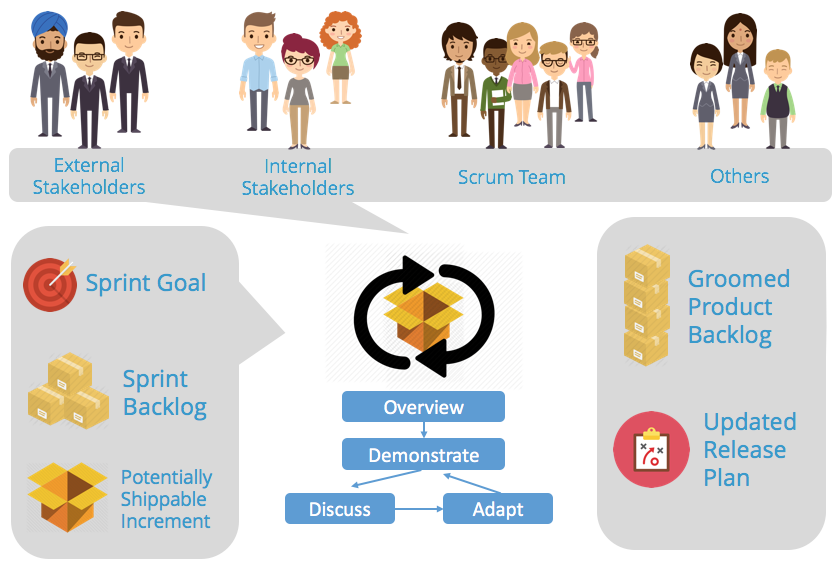
\includegraphics[scale=0.4]{images/sprint-review.png}
    \label{fig:revisao}
\end{figure}

\subsection{Objetivo}

O objetivo dessa reunião é, como listado por \citet{Adkins2010Coaching}:

\begin{itemize}[leftmargin=3em, noitemsep, nosep, before=\vspace{1cm}, after=\vspace{1cm}]
    \setlength{\itemindent}{1em}
    \item \textbf{Demonstrar comprometimento}: O time relembra o objetivo definido ao inicio da \textit{sprint} e diz o que foi feito e o que não foi feito, além de pedir formalmente a aceitação do que foi feito para o \textit{PO};
    \item \textbf{Mostrar o produto}: O time mostra os objetivos que foram alcançados, sem slides bonitos ou oratória, mas sim com o produto funcionando;
    \item \textbf{Oferecer insights}: O time oferece a sua visão de como o time está trabalhando entre si e no contexto da organização para os \textit{stakeholders};
    \item \textbf{Pedir ajuda}: Além das atividades anteriores, o time também pode trazer a tona impedimentos que o \textit{PO} ou o ScrumMaster não podem resolver.
\end{itemize}

\subsection{Papel do ScrumMaster}

Durante a reunião de revisão da \textit{sprint}, o ScrumMaster não é importante, geralmente sentando longe da ação. Por outro lado, isso não significa que ele ficará dormente durante toda a reunião. Enquanto o time toma a frente e mostra o produto, o ScrumMaster faz observações e anotações sobre os seguintes pontos:

\begin{enumerate}[leftmargin=3em, noitemsep, nosep, before=\vspace{1cm}, after=\vspace{1cm}]
    \setlength{\itemindent}{1em}
    \item Como os membros do time estão interagindo? Eles dão atenção e suporte para quem está falando? Eles olham para quem está falando? Eles estão fazendo outra coisa enquanto estão na reunião?
    \item Como o time está interagindo com o \textit{PO}, cliente ou com outros \textit{stakeholders}?
    \item O \textit{PO} utilizou o \textit{backlog} do produto como uma maneira de gerenciar os pedidos ou mudanças de prioridade que recebeu?
    \item Os membros do time passaram a palavra entre si tranquilamente? Todos que queriam falar conseguiram?
    \fonte{\cite{Adkins2010Coaching}}
\end{enumerate}

As observações feitas sobre a utilização de práticas ágeis acabarão caindo em duas classes: as \enquote{\textbf{Good for you}}, representando as boas práticas que o time mostrou na reunião, e as \enquote{\textbf{Ops, deixaram escapar aquilo}}, que representam os deslizes do time em alguma prática ágil.

Após a reunião, o ScrumMaster deve oferecer compartilhar as suas observações. As observações em sinão precisam estar conclusivas ou polidas, só é necessário o que foi anotado. Com essas anotações, a equipe poderá entender melhor o que está acontecendo e ajudar o ScrumMaster a entender melhor o que está acontecendo.

É comum que, com o feedback fornecido pelo ScrumMaster, a equipe discuta sobre as observações. Também é possível que o time não ouça ou talvez ignore. Provavelmente o time estará cansado após a reunião de revisão, então só o fato de oferecer as observações já é o suficiente.

% Revisão da sprint %%%%%%%%%%%%%%%%%%%%%%%%%%%%%%%%%%%%%%%%%%%%%%%%%%%%%%%%%%%%%%

\section{Retrospectiva da sprint}

A reunião de retrospectiva da \textit{sprint} é o ponto culminante da iteração. Por convenção, é uma reunião que marca o final da iteração e que dura geralmente 1 hora, mas que pode durar mais caso algum tópico importante entre em discussão. Todo o time, incluindo \textit{PO} e, claro, ScrumMaster devem participar. A Figura \ref{fig:retro} exemplifica a estrutura básica de uma retrospectiva de iteração.

\begin{figure}[htbp]
    \centering
    \caption{Exemplo da estrutura de uma reunião de retrospectiva.}
    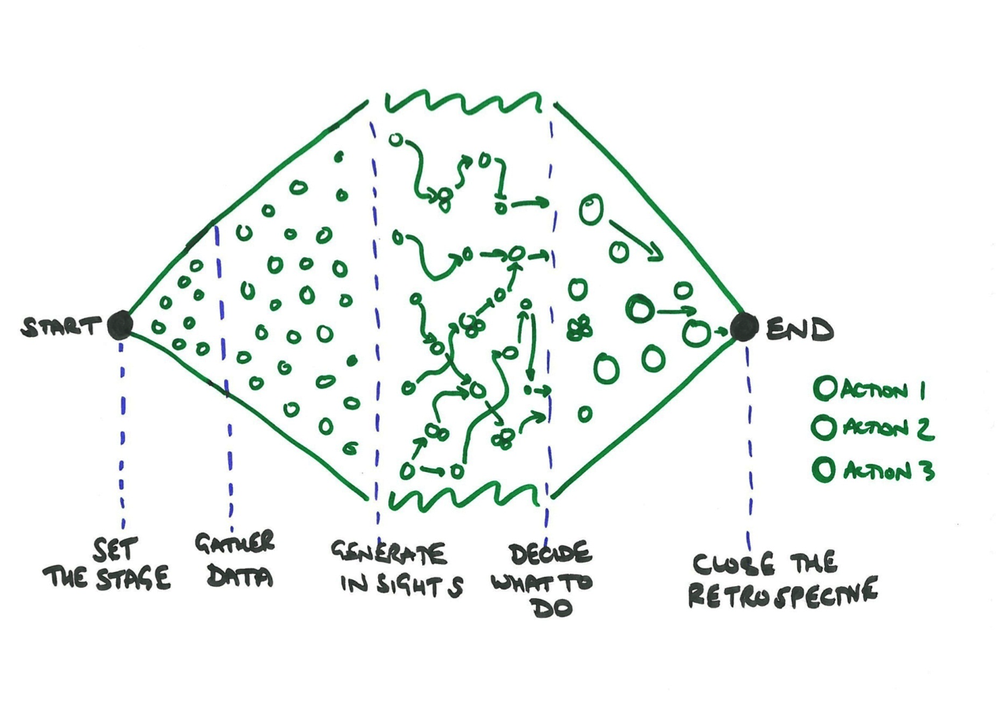
\includegraphics[scale=0.8]{images/retro-structure.png}
    \label{fig:retro}
\end{figure}

\subsection{Objetivo}

Como listado por \citeauthor{Adkins2010Coaching}, a reunião de retrospectiva da iteração tem como objetivos:

\begin{itemize}[leftmargin=3em, noitemsep, nosep, before=\vspace{1cm}, after=\vspace{1cm}]
    \setlength{\itemindent}{1em}
    \item \textbf{Inspecionar e adaptar}: A retrospectiva é a hora de parar a ação, o que oferece ao time a oportunidade de respirar e de se perguntar o que aconteceu durante a iteração;
    \item \textbf{Analise o como, não o oque}: Na reunião, o time deve considerar como o trabalho foi feito, não somente o que foi feito nem o quão bom ficou, mas sim como o time trabalhou em conjunto para atingir o objetivo;
    \item \textbf{Se sair ainda melhor próxima vez}: O objetivo final dessa reunião é firmar um compromisso a fazer certas coisas diferentemente para se sair melhor ainda da próxima vez. Melhorar pode ser qualquer coisa que importa para o time, como, por exemplo, ser mais rápido ou aumentar o compromisso de todos os envolvidos.
\end{itemize}

\subsection{Papel do ScrumMaster}

Enquanto a iteração acontece, o ScrumMaster deve fazer várias observações sobre como o time está trabalhando junto--o que vai bem, o que parece estranho, o que está nebuloso. O ScrumMaster pode trazer esses pontos ao time quando eles aparecerem, mas, a não ser que seja um problema realmente mortal, ele deve provavelmente guardar as observações e trazê-las a tona durante a retrospectiva da \textit{sprint}. Isso garante que o time se preocupe com a tarefa em mão durante a iteração e não com como eles estão se comportando na iteração. Claro, o ScrumMaster deve considerar se esse time está aprendendo os princípios ágeis básicos ao tomar a decisão de guardar ou não suas observações. Algumas das observações que o ScrumMaster pode tomar são as seguintes:

\begin{enumerate}[leftmargin=3em, noitemsep, nosep, before=\vspace{1cm}, after=\vspace{1cm}]
    \setlength{\itemindent}{1em}
    \item O time está utilizando as estruturas fornecidas pela metodologia ágil para se manter coordenado?
    \item Como o time está aguentando a iteração?
    \item Como o trabalho está fluindo?
    \item Existem dificuldades na comunicação, coordenação, assiduidade, atenção ou colaboração?
    \item Em que momentos o time foi incrível?
    \item Quando o time parece lento, como se tivesse recém acordado?
    \item Como a ansiedade do time varia pela iteração?
    \item Como está cada membro fisicamente, mentalmente e emocionalmente?
    \item O quão animado o time fica em cada parte da iteração?
    \fonte{\cite{Adkins2010Coaching}}
\end{enumerate}

Quando a reunião se aproximar, o ScrumMaster deve revisar suas observações, talvez escolher um tema ou mais para focar na reunião. Também é interessante que o ScrumMaster procure a perspectiva de outros membros da equipe--perguntar o que eles viram, sobre o que eles estão curiosos, o que está incomodando eles. É importante que esse \textit{check-up} não vire uma mini atividade retrospectiva em si, logo o ScrumMaster deve deixar que a conversa seja superficial, somente uma pequena janela para a mente dos membros da equipe.

Durante a retrospectiva, o ScrumMaster deve novamente deixar claro que o time sabe a coisa certa a se fazer. Com isso dito, o ScrumMaster, ao iniciar a reunião, deve apresentar a agenda, quais atividades foram definidas para acompanhar os itens da agenda e, finalmente, pedir permissão ao time pela agenda.

O pedido de permissão geralmente seguirá a seguinte linha: \enquote{Vocês acreditam que essa agenda irá alcançar os objetivos nos quais essa reunião deveria focar?.} Nesse momento, o time pode decidir focar em coisas completamente diferentes do que as imaginadas pelo ScrumMaster, ou talvez pedir uma conversa mais informal, sem atividades. O time pode acabar estragando a reunião com a decisão, mas isso também é uma atividade de aprendizado.

Além disso tudo, o ScrumMaster também cuidará da duração da reunião, cronometrando de acordo com a duração definida a priori e avisando conforme o horário combinado se aproxima. Ao término do \textit{timebox}, o ScrumMaster anuncia o término da retrospectiva, mas, se o time quiser continuar, ele deve deixar desde que todos os membros do time queiram e desde que a duração extra também seja bem definida e \textit{timeboxed}. Ao término da reunião retrospectiva, o ScrumMaster pode convidar o time a escrever o que o time se comprometeu a fazer para a próxima reunião em papel, e deixar esse documento em algum lugar comum a todos.

Na próxima iteração, é importante manter esses compromissos em cheque, logo o ScrumMaster deve atentar se eles estão sendo seguidos pelo time ou se eles foram esquecidos. Nesse caso, traga à tona a falta de comprometimento do time com o que foi acordado várias vezes pela \textit{sprint}. Sempre que alguém seguir o acordo da última retrospectiva, mostre ao time o exemplo que esta pessoa está dando. Dê crédito em público para ela. Talvez o acordo da retrospectiva eventualmente fique esquecido. Em breve, alguém irá descumprir o acordo, e o time sentirá o efeito. Nesse caso, o ScrumMaster não pode deixar essa infração passar em branco. Ele pode perguntar: \enquote{Gente, o que aconteceu com o que combinamos na última retrospectiva sobre não fazer mais isso?}

Ademais, o ScrumMaster deve procurar oportunidades de lembrar o time sobre o que foi acordado na última retrospectiva. Ao fazer isso, provavelmente o time começará a fazer isso por conta própria e não deixará o que foi acordado ser esquecido.

\section{Conclusão}

Como observado nas seções anteriores, todas as reuniões definidas pelo Scrum como atividades de introspecção, retrospecção e de planejamento são, essencialmente, o núcleo da melhoria constante. Todo o propósito de uma metodologia incremental iterativa é gerar feedback e agir--melhorar--baseado nesse feedback. Isso gera comprometimento e melhora todos os aspectos de qualquer esforço de desenvolvimento em grupo.


%%%%%%%%%%%%%%%%%%%%%%%%%%%%%%%%%%%%%%%%%%%%%%%%%%%%%%%%%%%%%%%%%%%%%%%%%%%%%%%
% Reuniões
%

\chapter{Atividades}

Nesse capítulo, apresentarei algumas atividades que podem ser feitas como parte da agenda de uma reunião de retrospectiva da iteração como um método de melhorar o aproveitamento e aumentar os resultados da retrospectiva.

\section{Check-In}

Após introduzir a agenda da retrospectiva, cada membro do time deve responder uma breve pergunta feita pelo líder da retrospectiva com somente uma palavra. Essa atividade é feita para \enquote{preparar o palco} da reunião. Alguns exemplos de pergunta são:

\begin{itemize}[leftmargin=3em, noitemsep, nosep, before=\vspace{1cm}, after=\vspace{1cm}]
    \setlength{\itemindent}{1em}
    \item Quais são suas esperanças para essa retrospectiva?
    \item Qual é a palavra que descreve o que você precisa dessa reunião?
    \item Diga uma coisa que está na sua mente;
    \item Se você fosse um carro e estivesse vindo para essa retrospectiva, qual carro você seria?
    \fonte{\cite{Derby2006Retrospectives}}
\end{itemize}

Aquele que organizar a agenda da retrospectiva deve escolher uma pergunta com antecedência.

\section{Mad Sad Glad}

Essa atividade traz os sentimentos que o time teve à tona e serve para coletar dados emocionais sobre a iteração.

Nela, o líder da retrospectiva traz 3 folhas A2 rotuladas com \enquote{Mad}, \enquote{Sad} e \enquote{Glad}. Então o líder pede que cada membro escreva eventos em \textit{post-it}'s que os fizeram sentir felizes, nervosos e tristes na respectiva folha A2. Após 25 minutos, começe a perguntar ao grupo se certos cartões são similares, e então os agrupe. Após isso, faça as seguintes perguntas:

\begin{itemize}[leftmargin=3em, noitemsep, nosep, before=\vspace{1cm}, after=\vspace{1cm}]
    \setlength{\itemindent}{1em}
    \item O que salta aos olhos quando vocês olham para estes cartões?
    \item O que vocês acharam inesperado sobre os cartões?
    \item Quais são os padrões que emergiram?
    \item O que esses cartões sugerem como próximos passos a tomar?
    \fonte{\cite{Derby2006Retrospectives}}
\end{itemize}

\section{Fishbone}

Essa atividade traz à tona as causas de um problema e serve pra gerara insights sobre a iteração, entrega ou retrospectiva.

Inicialmente, o líder desenha um diagrama de espinha de peixe conforme a Figura \ref{fig:fishbone} e faz perguntas no modelo \enquote{Quais são os problemas da <categoria> causando ou afetando o problema <problema>?} para cada categoria. Então, o líder escreve as respostas ao redor do osso correspondente, adicionando novas espinhas conforme necessário. O time então deve analizar as respostas coletadas ao redor das espinhas para decidir quais medidas tomar para resolver esse problema.

\begin{figure}[htbp]
    \centering
    \caption{O diagrama de espinha de peixe.}
    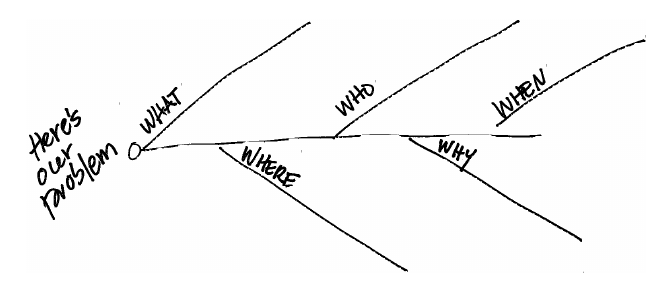
\includegraphics[scale=0.8]{images/fishbone.png}
    \label{fig:fishbone}
    \fonte{\cite{Derby2006Retrospectives}}
\end{figure}

%%%%%%%%%%%%%%%%%%%%%%%%%%%%%%%%%%%%%%%%%%%%%%%%%%%%%%%%%%%%%%

\bibliographystyle{abntex2-alf}
\bibliography{biblio} 

\end{document}
